This chapter describes our methodology to approach the problem of prediction of suicidality using machine learning algorithms.
First, we present the dataset used (the ELSA-Brasil study) and the steps adopted during its cleansing.
Next, we describe our model-induction pipeline for a set of supervised learning algorithms of interest.
Finally, we explain our strategies for model evaluation and for building an ensemble classifier.

Our proposal to approach the problem of prediction of suicidality can be summarized in three steps.
First, the data (in our case, from the \textit{ELSA-Brasil} study) is cleansed and minimally prepared.
Afterward, it is used by a model-induction pipeline, for a set of supervised learning algorithms of interest.
Finally, the models are evaluated and combined in an ensemble (which is also evaluated in the same manner).


\section{Dataset}\label{sec:dataset}

The Brazilian Longitudinal Study of Adult Health (ELSA-Brasil) dataset is a cohort of Brazilian adults (public universities' employees) in a longitudinal study with a follow-up of about 4 years~\cite{Schmidt2015, Aquino2012}.
Up to now, two waves of interviews and examinations have been conducted: the first from 2008 to 2010, the second from 2012 to 2014~\cite{Olivera2017}.
The baseline assessment included 15105 participants, with about 3000 assessed variables (although the availability of the attributes is restricted depending on the application).
Given the scope and context of our application, after requesting data access with the interest of investigating suicidality, a version of the ELSA-Brasil dataset was made available to this study that includes 2288 "baseline" features.

Moreover, the ELSA-Brasil study assessed non-psychotic psychiatric morbidity using the Clinical Interview Schedule-Revised (CIS-R) ~\cite{Nunes2016, Lewis1992}, which makes available information regarding depressive and/or suicidal thoughts on the cohort.
The full version of the applied CIS-R questionnaire is made available in annex ~\ref{ch:cis-r}.
Although the full array of 176 questions is not explored in this section, the ones found to be of most importance are discussed in Chapter~\ref{ch:experiments-and-results}.

In our work, we analysed only the first wave of the study and focused on a specific population of the ELSA-Brasil dataset, corresponding to the individuals presenting any common mental disorders, indicated by the \textit{mentalvar\_A\_TMC} feature.
The reason for restricting the dataset is that our goal is not to develop a model that identifies the presence of suicidality in the general population, as this would have limited utility, but rather to identify this condition for a population at risk.
Individuals with CMD are probably under the assistance of mental health professionals, who could act upon the suggestion of machine learning classifiers that the patient is prone to suicidal ideation and, by proxy, suicide attempts.
Besides, we also avoid broadening too much the training dataset to the point where class imbalance becomes too severe to handle, as the prevalence of suicidality is about 8.53\% in this cohort.
Although there is a clear trade-off between the ratio of instances in the positive class and the total number of instances in the training data, we apply this restriction since in our domain it is indispensable to make correct predictions for the positive class.
As a result of excluding the instances without CMD, our number of data points is reduced from 15105 to 4039, incurring the loss of 169 (13.11\%) positive class instances, but raising the probability of the class from 8.53\% to 27.73\%.

\subsection{Input Variables - Features}\label{subsec:features}

Besides socio-demographic and economic attributes, the ELSA-Brasil study assessed the participants' health in different aspects and means, from electrocardiograms to retinal photographs and mental health questionnaires~\cite{Schmidt2015}.
The available data in ELSA-Brasil includes attributes previously described in the literature as associated with suicide ideation, including gender, age, marital status~\cite{Nock2008}, socioeconomic status~\cite{Gunnell2009, Meltzer2012, Meneghel2004}, physical activity, alcohol consumption, self and family education levels~\cite{Souza2010a} and emotional difficulties (e.g.\ deaths of close relatives), social capital variables, pain conditions, chronic diseases, obesity and body mass index, the existence of physical disabilities~\cite{Meltzer2012a}, and sexual orientation~\cite{Silenzio2007}.

As predictors of our models, we used all 2288 variables from the baseline dataset.
Besides, we also included variables from the CIS-R questionnaire, which, after excluding the variables used as outcomes, consists of 173 variables.
Therefore, the total number of predictors before data cleansing was 2461 features.

\subsection{Outcome Variables - Labels}\label{subsec:labels}

To represent the concept of suicidality, which is the outcome of our classifiers (i.e.\ a binary factor indicating the presence or absence of suicidality for a given instance), we assess and combine hopelessness, "taedium vitae", and suicidal ideation in logical disjunction, a boolean \textit{OR}.
These variables are, respectively, indicated by the responses to the CIS-R's H6, H8, and H9 questions:
\begin{itemize}
    \item CIS-R H6 (hopelessness): \textit{Have you felt hopeless at all during the past seven days, for instance about your future?}
    \item CIS-R H8 (taedium vitae): \textit{In the past week have you felt that life isn't worth living?}
    \item CIS-R H9 (suicidal ideation): \textit{In the past week, have you thought of killing yourself?}
\end{itemize}

Although the formulation of the questions implies a naturally binary "yes or no" response, both H8 and H9 have a third option, which is of presenting taedium vitae or suicidal ideation but not exactly in the last 7 days.
To this study, the third-option responses are considered as positive ones (i.e., as if the person had responded to the questions with a "yes").
These variables had several missing values since the majority of the interviewees did not reach the point of being asked their respective questions - they responded negatively to prior ones that are more general, such that we can assume there is an implicit negative answer to the more specific ones which we are interested.
Thus, absent values for CIS-R's H6, H8, and H9 variables were inferred as negative entries.

\subsection{Data Cleansing}\label{subsec:cleansing}

As a stride in the direction of improving data quality for the induction of the models, it is desirable to validate and clean (or \textit{wrangle}) the data before usage.
~\citet{Kandel2011} describe data wrangling and analysis as an iterative process consisting of cleansing, merging, adapting, and evaluating the data.

Considering that the ELSA-Brasil study has several variables obtained by non-linear interviews (skipping questions depending on answers), some instances present missing values.
Although our methodology includes a mechanism for inference of unavailable (NA) values (see Section ~\ref{sec:preproc-train-eval}), we considered important for data fidelity and for model quality to leave aside variables that have more NAs than a certain threshold - which we set as 10\% in this study.

Our solution does not include any natural language processing techniques, thus all free-text variables in ELSA-Brasil were removed.
We provide a list of textual variables removed in Table~\ref{tab:free-text-removed}.

Finally, and perhaps most importantly, given the chosen CIS-R questions (H6, H8, and H9) to be combined into our outcome label, we removed the predictors that indirectly make use of these variables - except for \textit{mentalvar\_A\_ESCORETOTAL}, which is adapted to be the sum of the numerical value of answers in the CIS-R H section excluding H6, H8, and H9.
These are, in the dataset, the variables shown in Table~\ref{tab:removed-info-leak}.
This step is crucial to avoid data leakage in model training, where our input variables (i.e.\ predictors) would improperly contain information about the outcome to be predicted.

\begin{table}[h]
    \caption{Attributes removed for introducing information leakage}
    \begin{center}
        \begin{tabular}{l|l}
            \textit{Attribute}           & \textit{Description}                     \\
            \hline
            \hline
            mentalvar\_\_TMAD            & Mixed anxiety-depressive disorder (MADD) \\
            mentalvar\_a\_DEP            & Major depressive disorder (MDD)          \\
            mentalvar\_A\_DEPGRAVE       & Severe MDD                               \\
            mentalvar\_A\_DEPLEVCSINT    & Mild MDD with somatic symptoms           \\
            mentalvar\_A\_DEPLEVSSINT    & Mild MDD no somatic symptoms             \\
            mentalvar\_A\_DEPMODCSINT    & Moderate MDD with somatic                \\
            mentalvar\_A\_DEPMODSSINT    & Moderate MDD no somatic                  \\
            mentalvar\_A\_ESCORETOTAL    & CMD score (continuous)                   \\
            mentalvar\_A\_SINTIDEIADEP   & Depressive thoughts symptoms             \\
            mentalvar\_A\_TMC            & Common Mental Disorder (CMD) (bin)       \\
            mentalvar\_A\_TMCGRAV        & Common Mental Disorders (CMD) (3 levels) \\
            mentalvar\_MDD\_trajectories & group(a\_DEP b\_DEP)                     \\
            mentalvar\_only\_incident    & Incident MDD                             \\
            mentalvar\_only\_remitted    & Remitted MDD                             \\
            \hline
        \end{tabular}
    \end{center}
    \legend{Source: The Author}
    \label{tab:removed-info-leak}
\end{table}

Upon removal of these variables, it is desirable to supply the models with some sensible substitute to the data that was taken away, since the variables were of great importance for the clinical diagnosis of suicidality.
Since interpretations of responses to the H section of CIS-R were summarized in the removed features, the idea is that the learners would instead interpret these relations by themselves given the necessary data.
Thus, our cleansing needs steps to also impute missing values in CIS-R answers, which were frequent given the interview is non-linear, so they are not removed by our afore-mentioned 10\%-maximum NA filter.
For this task, we realized that the majority of the answers could be reliably inferred from the context, if the person responded negatively to a question X, then some question Y which only makes sense if X was answered positively can be inferred to be negative too.

In conclusion, because of absent values, textual input, and information leakage, our cleansing procedure reduces the number of predictors to be employed in the model-fitting process, represented in Table~\ref{tab:dataset-cleansing}, and does not change the number of instances in the data.
The final high-level quantitative characteristics of our dataset are summarized in Table~\ref{tab:final-dataset-characteristics}.

\begin{table}[h]
    \caption{Number of variables in light of dataset cleansing process}
    \begin{center}
        \begin{tabular}{c|c}
            \textit{Attribute Set}        & \textit{Set Size}       \\
            \hline
            \hline
            Total (uncleansed)            & 2463 (100\%)            \\
            Removed (information leakage) & 13 (0.69\%)             \\
            Removed (NA excess)           & 773 (31.38\%)           \\
            Removed (free-text)           & 47 (1.91\%)             \\
            \textbf{Remaining (cleansed)} & \textbf{1626 (66.02\%)} \\
            \hline
        \end{tabular}
    \end{center}
    \legend{Source: The Author}
    \label{tab:dataset-cleansing}
\end{table}

\begin{table}[h]
    \caption{Main quantitative characteristics of cleansed dataset}
    \begin{center}
        \begin{tabular}{c|c}
            \textit{Dataset Characteristic} & \textit{Value} \\
            \hline
            \hline
            \#Instances                     & 4039           \\
            \#Attributes                    & 1626           \\
            \#Positives                     & 1120 (27.73\%) \\
            \#Negatives                     & 2919 (72.27\%) \\
            \hline
        \end{tabular}
    \end{center}
    \legend{Source: The Author}
    \label{tab:final-dataset-characteristics}
\end{table}


\section{Pre-processing, Training, and Evaluation}\label{sec:preproc-train-eval}

The goals in the proposed approach to produce our learners are: to attain interpretability and prediction performance.

With this goal in mind, we define our methodology considering the particularities of our dataset that make the development of predictive models particularly challenging.
The adopted dataset is highly skewed towards a majority class of non-suicidal instances, such that our procedures require the usage of techniques to mitigate class imbalance biases and to appropriately evaluate model performance in such a scenario.
There is also the problem of having numerous features for each instance, which can make it harder for the learners to have both good predictive qualities and interpretability.

\subsection{Pipeline and Pre-Processing}\label{subsec:pipeline-and-preprocessing}

The ordered combination of the main steps of our approach is summarized in the three-staged pipeline diagram of Figure~\ref{fig:train-pipeline}.
The highest layer, of evaluation, encompasses the whole cleansed dataset and orchestrates the fitting of models (abstracted by lower layers) and their performance assessment for each supervised learning algorithm.
The RFE procedure has its own layer (in blue), where the data is each training fold of the evaluation phase (also in blue), so the final test data is never used in induction.
Finally, within the scope of the yellow data boxes, the RFE models training folds, the most basic supervised learning layer (also in yellow) induces classifiers with hyperparameter tuning.

To avoid data leakage in the base learners induction, pre-processing is only applied in the lowest layer of our pipeline.
If pre-processing were applied before, the training data in the lowest layer would have been processed in a manner that uses information from its corresponding test data.
In this undesirable scenario, we could expect to have models with optimistic performance estimates that would perform (drastically) differently upon inferences on new data.

\begin{figure}[]
    \caption{Preprocessing, training and evaluation pipeline}
    \centerline{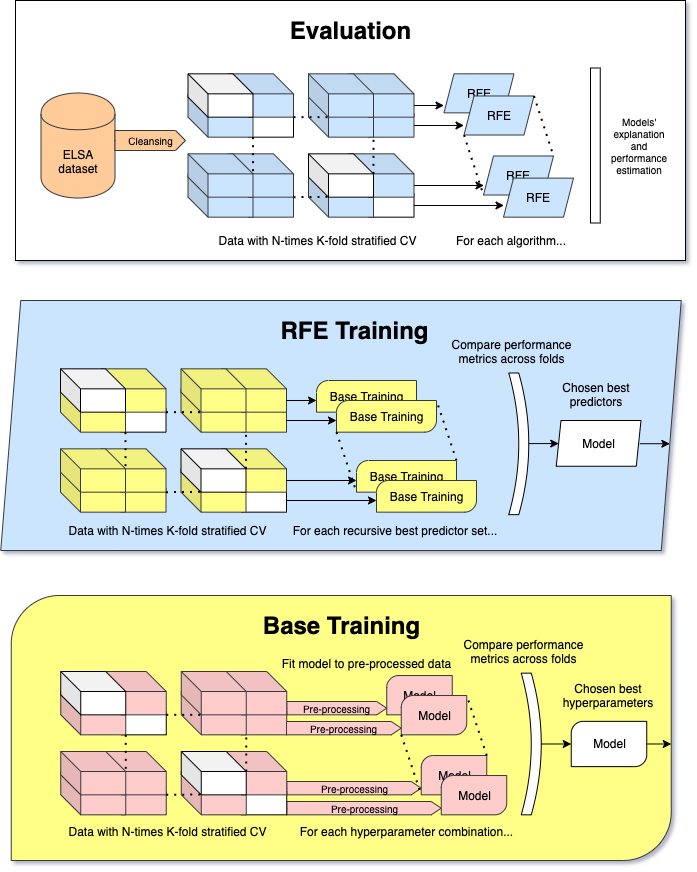
\includegraphics[scale=.6]{fig_pipeline_diagram}}
    \label{fig:train-pipeline}
    \legend{Source: Author}
\end{figure}

The preprocessing itself is proposed to be a sequential application of the following steps, each parameterized and described as general procedures:
\begin{itemize}
    \item \textbf{downsampling}, removing negative instances until the class distribution is of a given ratio (e.g.,\ 2N:1P, 3N:2P, etc - but not 1:1);
    \item \textbf{NA imputation}, inferring missing values using a function of the respective predictor values (e.g.\, the mean, or some classification or clustering ML technique, etc.);
    \item \textbf{near-zero variance (NZV) cut}, excluding useless predictors with a uniformity of values, defined by a parameterized quantitative criteria (e.g\, frequency distribution thresholds);
    \item \textbf{high-correlation filtering}, removing variables that are highly correlated to others (i.e.\ with correlation over a threshold) and that do not present distinct and useful information;
    \item \textbf{SMOTE}, synthetically creating positive instances derived from a fixed number of nearest neighbors (e.g.\ 3, 5, 7 etc) until the class distribution is of a given ratio (e.g.\ 1:1), (nearly) balancing the ratio of observations per class.
\end{itemize}

Note that the pre-processing steps of the pipeline do not necessarily promote perfect class balance for subsequent model induction.
This is controlled by adjusting the parameters related to the balance ratio, taking into account whether the supervised learning algorithm by itself can deal with the class imbalance to some extent.

\subsection{Model Induction Approach}\label{subsec:model-induction-approach}

We also aim to reduce the number of attributes of the data used in training and predictions to have a more interpretable classifier, from which clinicians can obtain intuitive knowledge.
In our work, we applied RFE to wrap "base learners" in a feature selection loop, where a model will have as the final predictor set the one that yielded the highest F\textsubscript{2}-Score.
Each iteration of feature elimination retrains the model and reassesses the variable importances rank so that only the best predictors are carried on to the next induction.
Again, to avoid selection bias~\cite{Ambroise2002, Reunanen2003} and for the other reasons presented in~\ref{subsec:performance-assessment-approach}, the feature elimination procedure must be embedded in an N-times K-fold stratified cross-validation.

Finally, the essential and basic supervised learning procedure (which is wrapped in RFE) makes use of hyperparameter tuning by grid search (GS), where we select optimal models by performance comparisons (again, using the F\textsubscript{2}-Score) of inductions done with several combinations of hyperparameters.
Another cross-validation of the same sort as the ones just described must be applied here, for the same reasons.

\subsection{Performance Assessment Approach}\label{subsec:performance-assessment-approach}

The F\textsubscript{2}-Score is used as the optimization metric during model induction and as the main evaluation metric.
In the latter case, other values are also calculated to estimate the generalization power of the classifier: the area under the ROC curve (AUCROC), the sensibility, and the specificity.

The F\textsubscript{2}-Score is chosen as the most relevant measure not only for its intuitive meaning of valuing the positive class more than the negative one (which is essential for a suicide ideation classification, where the false negatives errors are the most costly) but also because it forces models not to sacrifice precision.
This metric is often neglected in favor of specificity, thus in many cases being, without notice, quite low while the other is high.
It shows possible deficiencies of having many errors in the positive predictions, while specificity shows whether we have correctly found the true negatives within the negative instances.
Thus, although the positive class requires the highest attention in our study, we must also assess both specificity and precision.

With a zeal for realistic and statistically-robust estimates of real-life performance, we employed a stratified N-times K-fold CV to separate our data, in our final evaluation mechanism.

\subsection{Ensemble Composition}\label{subsec:ensemble-composition}

\begin{figure}[h]
    \caption{Weighted-averaging ensemble constitution and evaluation}
    \centerline{\includegraphics[scale=.3]{../notes/ensemble-diagram/ensemble.png}}
    \label{fig:ensemble}
    \legend{Source: Author}
\end{figure}

Lastly, our approach includes the composition of multiple models trained with different algorithms or pipeline parameters in an ensemble.
This model is not trained by itself as a whole, its constituents are trained separately.
For each CV resample of the pipeline's highest layer, the trained models simply have their inference outputs combined by weighted averaging of the classification probability, as illustrated in Figure~\ref{fig:ensemble}.
The idea is that the ensemble can compensate or mitigate each models' particular difficulties and consolidate their consensus.
For that, it is desirable to make use of algorithms that provide this variability and diversity, although the nature of the pipeline already introduces a great mechanism of differentiation through RFE, such that models are not fit over the same predictors.


